\section{A Real-coded Parallel Genetic Algorithm on the GPU}
\subsection{Algorithm Overview}
\frame
{
\frametitle{A Real-coded Parallel Genetic Algorithm on the GPU}
\framesubtitle{Algorithm Overview}
\begin{itemize}
	\item \blue{Fine-grained} parallel model.
	\item 2D toroidal grid as the spatial \blue{population structure} where each grid point contains one individual.
	\item The neighborhood defined on the grid always contains \red{5 individuals}.
\end{itemize}
}

\frame
{
\frametitle{A Real-coded Parallel Genetic Algorithm on the GPU}
\framesubtitle{Algorithm Overview}
\begin{center}
	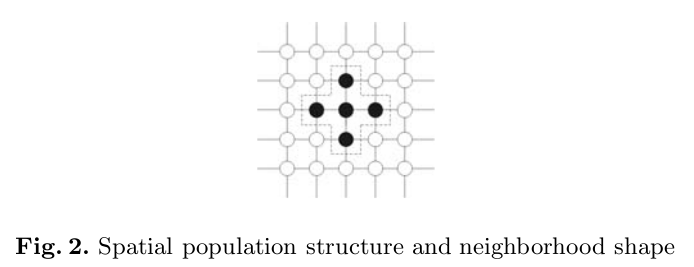
\includegraphics[width=0.8\textwidth]{img/vecinos}
\end{center}
}

\frame
{
\frametitle{A Real-coded Parallel Genetic Algorithm on the GPU}
\framesubtitle{Algorithm Overview}
\begin{itemize}
	\item \red{Crossover operator}.
	\item For each individual (best individual + itself).
	\item Several crossover operators can be defined (averaging, uniform, blend)
	\item \blue{Blend crossover} is used, two chromosomes selected...\blue{randomly} selects a value for each offspring gene $y_i$, using distribution within the range:
	$$\left[C_{min} + \alpha \cdot I, C_{max} - \alpha \cdot I\right]$$ 
	$$ C_{min} = min\{x_{i}^{1}, x_{i}^{2}\},\ C_{max} = max\{x_{i}^{1}, x_{i}^{2}\}$$
	$$ I = C_{max} - C_{min},\ \alpha, \text{tunable parameter} $$
\end{itemize}
}

\frame
{
\frametitle{A Real-coded Parallel Genetic Algorithm on the GPU}
\framesubtitle{Algorithm Overview}
\begin{itemize}
	\item \red{Mutation operation} (final step)
	\item \blue{Role}, restore lost or unexpected genetic material. (preventing premature convergence)
	\item Here, a \blue{non-uniform mutation} is adopted.
\end{itemize}
}

\frame
{
\frametitle{A Real-coded Parallel Genetic Algorithm on the GPU}
\framesubtitle{Algorithm Overview}
\begin{itemize}
	\item If is applied at generation step $t$ of $tmax$, the new value of the $i-th$ gene will be:
    \[
    y_{i} = \left\{ 
        \begin{array}{l l}

		x_{i} + \delta \cdot (U_{i} - x_{i}) & \text{if $\tau$ = 0}\\
		x_{i} - \delta \cdot (x_{i} - L_{i}) & \text{if $\tau$ = 1}\\
        \end{array} \right.
    \]
	\item where $\tau$ is random 0 or 1.
	\item $L_{i}$ and $U_{i}$ are the lower and upper bound of $x_{i}$ and:
	$$\delta = 1 - r^{(1-\frac{1-t}{t_{max}})^{b}}$$
	\item $r$ (random [0,1]), $b$ is user parameter
\end{itemize}
}
\subsection{Representation of Population}
\frame
{
\frametitle{A Real-coded Parallel Genetic Algorithm on the GPU}
\framesubtitle{Representation of Population}
\begin{itemize}
	\item We need to \red{represent} the population data in a \blue{format} that is \blue{accessible} by the GPU.
	\item General idea, \blue{store} population in a set of \emph{texture maps} and implement genetic operators.
	\item In our representation, chromosome \blue{sequentially divided} (segments) distributed in a number of \blue{textures} with the same position.
\end{itemize}
}

\frame
{
\frametitle{A Real-coded Parallel Genetic Algorithm on the GPU}
\framesubtitle{Representation of Population}
\begin{center}
	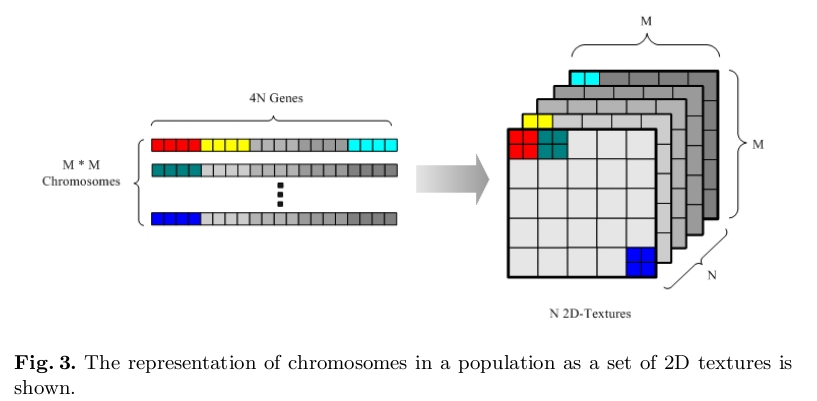
\includegraphics[width=0.8\textwidth]{img/representation}
\end{center}
}

\frame
{
\frametitle{A Real-coded Parallel Genetic Algorithm on the GPU}
\framesubtitle{Representation of Population}
\begin{itemize}
	\item Every segment contains \blue{four genes} packed into a \red{single pixel} RGBA channels. (population textures)
	\item Fitness textures.
	\item Advantages
	\begin{itemize}
		\item Keeps \blue{2D grid} topology of the population
		\item Fragment programs of genetic operators only \blue{need} to look-up considered \blue{pixel} (keeps the memory cache)
		\item \blue{Packing} of four genes (use of the wide SIMD).
		\item Four times (genes) can be processed \blue{simultaneously}.
	\end{itemize}
\end{itemize}
}

\subsection{Fitness Evaluation}
\frame
{
\frametitle{A Real-coded Parallel Genetic Algorithm on the GPU}
\framesubtitle{Fitness Evaluation}
\begin{itemize}
	\item This framework \blue{is designed} for solving problems whose fitness function can be implemented \red{entirely} in GPU.
	\item To avoid the \blue{bottleneck} (reading population from graphics hardware).
	\item Fitness GPU $>$ fitness CPU.
	\item Fitness evaluation by fragments program. 
\end{itemize}
}
\subsection{Random Numbers Generator}
\frame
{
\frametitle{A Real-coded Parallel Genetic Algorithm on the GPU}
\framesubtitle{Random Numbers Generator}
\begin{itemize}
	\item Current graphics hardware \blue{does not} provide the function to generate random numbers.
	\item We use a Linear Congruential Generator (LCG):
	$$I_{j+1} = a\cdot I_{j} + c (mod m)$$
\end{itemize}
}
\subsection{Genetic Operators}
\frame
{
\frametitle{A Real-coded Parallel Genetic Algorithm on the GPU}
\framesubtitle{Genetic Operators}
\begin{itemize}
	\item Selection, crossover and mutation operators can \blue{easily mapped} to a single fragment program.
	\item These fragments needs look-up \emph{population textures}, \emph{fitness textures} and \emph{random textures}.
	\item This result is written into a \blue{new} population texture
	\item In each rendering pass, four genes of each chromosome are processed parallelled.
	\item Crossover and Mutation operator used on \blue{independent} gene.
\end{itemize}
}
